\documentclass[12pt]{article}
\usepackage{graphicx}
\usepackage[]{mcode}
\usepackage{amsmath}
\usepackage[T1]{fontenc}
%\usepackage{lingmacros}
%\usepackage{tree-dvips}
%\usepackage{blindtext}
%\usepackage[utf8]{inputenc}

\renewcommand{\thesubsection}{\thesection.\alph{subsection}}

\begin{document}

\title{CMSC 460 - HW3}
\author{Gudjon Einar Magnusson}

\maketitle

\section{} %3.3

\subsection{}

Figure \ref{fig_interp_plot} shows interpolated value of $x$ and $y$ using each of the interpolation methods.

\begin{figure}
    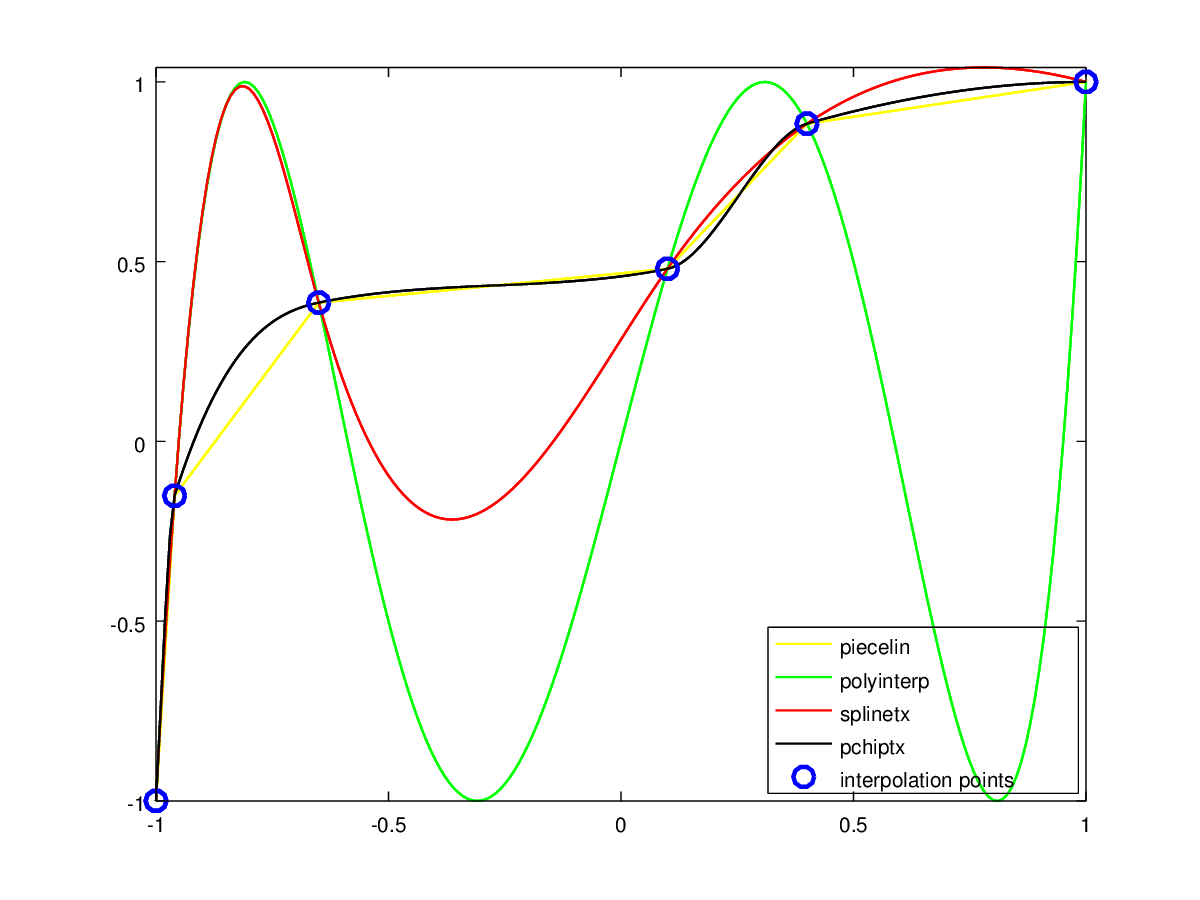
\includegraphics[width=\linewidth]{interp_plot}
    \centering
    \caption{4 different ways to interpolate between 6 points}
    \label{fig_interp_plot}
\end{figure}

\subsection{}

For each of the interpolation methods I evaluated the function at $x = -0.3$. In this case I prefer the result of \textit{pchiptx}. Its smooth and makes minimal assumptions about the shape of the function.
\begin{description}
    \item[piecelin] \hfill \\
    $p(-0.3) = 0.42996$
    \item[polyinterp] \hfill \\
    $p(-0.3) = -0.999$
    \item[splinetx] \hfill \\
    $p(-0.3) = -0.1957$
    \item[pchiptx] \hfill \\
    $p(-0.3) = 0.43218$
\end{description}

\subsection{}


\section{} %3.4

\section{} %3.7

\end{document}